% Three-Destination Sorting Model — TikZ Diagram
% Three panels stacked vertically, publication-ready

\begin{figure}[t]
\centering
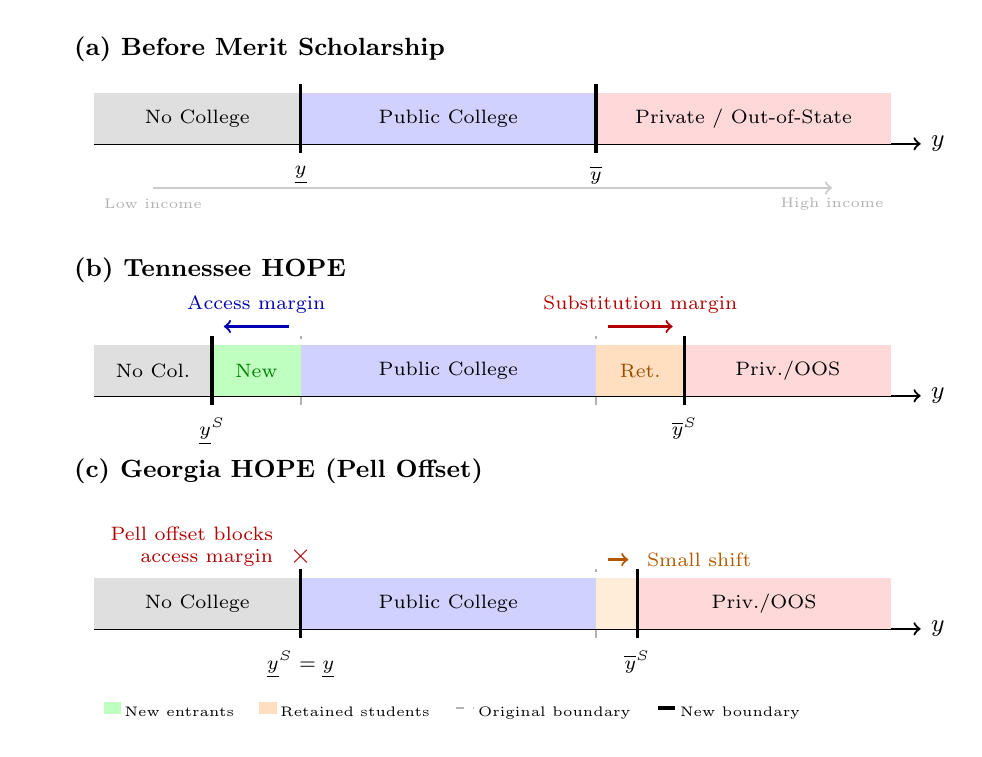
\begin{tikzpicture}[
  x=0.75cm, y=0.8cm,
  region/.style={minimum height=0.7cm, text=black, font=\scriptsize},
  boundary/.style={thick, dashed, gray!60},
  newboundary/.style={very thick, black},
  panellabel/.style={font=\small\bfseries, anchor=west},
  legendbox/.style={font=\tiny, anchor=west},
]

% ============================================================
% Panel A: Pre-Scholarship  (y = 12 to 14)
% ============================================================
\node[panellabel] at (-0.5, 13.0) {(a) Before Merit Scholarship};

% Income axis
\draw[thick, ->] (0, 11.5) -- (14, 11.5) node[right, font=\small] {$y$};

% Shaded regions
\fill[gray!25] (0, 11.5) rectangle (3.5, 12.3);
\fill[blue!18] (3.5, 11.5) rectangle (8.5, 12.3);
\fill[red!15] (8.5, 11.5) rectangle (13.5, 12.3);

% Region labels
\node[region] at (1.75, 11.9) {No College};
\node[region] at (6, 11.9) {Public College};
\node[region] at (11, 11.9) {Private / Out-of-State};

% Boundaries
\draw[very thick] (3.5, 11.35) -- (3.5, 12.45);
\draw[very thick] (8.5, 11.35) -- (8.5, 12.45);
\node[font=\scriptsize, below] at (3.5, 11.3) {$\underline{y}$};
\node[font=\scriptsize, below] at (8.5, 11.3) {$\overline{y}$};

% Income gradient
\draw[gray!40, thick, ->] (1, 10.8) -- (12.5, 10.8);
\node[font=\tiny, gray!60] at (1, 10.55) {Low income};
\node[font=\tiny, gray!60] at (12.5, 10.55) {High income};

% ============================================================
% Panel B: Post-Scholarship (Tennessee)  (y = 6 to 9.5)
% ============================================================
\node[panellabel] at (-0.5, 9.5) {(b) Tennessee HOPE};

% Income axis
\draw[thick, ->] (0, 7.5) -- (14, 7.5) node[right, font=\small] {$y$};

% Original boundaries (dashed)
\draw[boundary] (3.5, 7.35) -- (3.5, 8.45);
\draw[boundary] (8.5, 7.35) -- (8.5, 8.45);

% Shaded regions
\fill[gray!25] (0, 7.5) rectangle (2, 8.3);
\fill[green!25] (2, 7.5) rectangle (3.5, 8.3);
\fill[blue!18] (3.5, 7.5) rectangle (8.5, 8.3);
\fill[orange!25] (8.5, 7.5) rectangle (10, 8.3);
\fill[red!15] (10, 7.5) rectangle (13.5, 8.3);

% Region labels
\node[region] at (1, 7.9) {No Col.};
\node[region, green!50!black] at (2.75, 7.9) {New};
\node[region] at (6, 7.9) {Public College};
\node[region, orange!60!black] at (9.25, 7.9) {Ret.};
\node[region] at (11.75, 7.9) {Priv./OOS};

% New boundaries
\draw[newboundary] (2, 7.35) -- (2, 8.45);
\draw[newboundary] (10, 7.35) -- (10, 8.45);
\node[font=\scriptsize, below] at (2, 7.3) {$\underline{y}^S$};
\node[font=\scriptsize, below] at (10, 7.3) {$\overline{y}^S$};

% Arrows showing shifts
\draw[thick, ->, blue!70!black] (3.3, 8.6) -- (2.2, 8.6);
\node[font=\scriptsize, blue!70!black, above] at (2.75, 8.65) {Access margin};

\draw[thick, ->, red!70!black] (8.7, 8.6) -- (9.8, 8.6);
\node[font=\scriptsize, red!70!black, above] at (9.25, 8.65) {Substitution margin};

% ============================================================
% Panel C: Georgia (Pell Offset)  (y = 1.5 to 5.5)
% ============================================================
\node[panellabel] at (-0.5, 6.3) {(c) Georgia HOPE (Pell Offset)};

% Income axis
\draw[thick, ->] (0, 3.8) -- (14, 3.8) node[right, font=\small] {$y$};

% Original boundary (dashed, upper only — lower doesn't move)
\draw[boundary] (8.5, 3.65) -- (8.5, 4.75);

% Shaded regions
\fill[gray!25] (0, 3.8) rectangle (3.5, 4.6);
\fill[blue!18] (3.5, 3.8) rectangle (8.5, 4.6);
\fill[orange!15] (8.5, 3.8) rectangle (9.2, 4.6);
\fill[red!15] (9.2, 3.8) rectangle (13.5, 4.6);

% Region labels
\node[region] at (1.75, 4.2) {No College};
\node[region] at (6, 4.2) {Public College};
\node[region] at (11.35, 4.2) {Priv./OOS};

% Boundaries
\draw[newboundary] (3.5, 3.65) -- (3.5, 4.75);
\draw[newboundary] (9.2, 3.65) -- (9.2, 4.75);
\node[font=\scriptsize, below] at (3.5, 3.6) {$\underline{y}^S = \underline{y}$};
\node[font=\scriptsize, below] at (9.2, 3.6) {$\overline{y}^S$};

% Blocked access — red X and annotation to the LEFT, not above
\node[font=\normalsize, red!70!black] at (3.5, 4.95) {$\boldsymbol{\times}$};
\node[font=\scriptsize, red!70!black, anchor=east, text width=3cm, align=right] at (3.2, 5.1)
  {Pell offset blocks\\access margin};

% Small substitution arrow and annotation to the RIGHT
\draw[thick, ->, orange!70!black] (8.7, 4.9) -- (9.05, 4.9);
\node[font=\scriptsize, orange!70!black, anchor=west] at (9.2, 4.9) {Small shift};

% ============================================================
% Legend
% ============================================================
\node[legendbox] at (0, 2.5) {%
  \tikz[baseline=-0.5ex]{\fill[green!25] (0,0) rectangle (0.3,0.18);}\,New entrants \quad
  \tikz[baseline=-0.5ex]{\fill[orange!25] (0,0) rectangle (0.3,0.18);}\,Retained students \quad
  \tikz[baseline=-0.5ex]{\draw[thick, dashed, gray!60] (0,0.09) -- (0.3,0.09);}\,Original boundary \quad
  \tikz[baseline=-0.5ex]{\draw[very thick, black] (0,0.09) -- (0.3,0.09);}\,New boundary
};

\end{tikzpicture}

\caption{Three-Destination Sorting: How Merit Scholarships Reshape
  Institutional Composition}
\label{fig:sorting_model}

\vspace{1mm}
\begin{minipage}{0.92\textwidth}
  \footnotesize
  \textit{Notes:} Panel~(a) shows pre-scholarship sorting by family
  income $y$. Panel~(b) shows Tennessee HOPE: the scholarship reduces
  the effective price of public college, shifting the lower boundary
  left (access margin: low-income students enter) and the upper boundary
  right (substitution margin: high-income students retained in public
  rather than exiting to private). The public sector expands in both
  directions, producing progressive sorting. Panel~(c) shows Georgia
  HOPE: the Pell offset eliminates the effective subsidy for
  bottom-quintile families, so the lower boundary does not shift
  ($\times$). Only the upper boundary moves modestly, producing
  regressive sorting.
\end{minipage}
\end{figure}
